\documentclass{beamer}
\mode<presentation>{
	\usetheme{Warsaw}%{CambridgeUS}
	%\usecolortheme{sidebartab}
	%\usecolortheme{spruce}
	\usepackage{color}
	\definecolor{celeste_ucr}{RGB}{65,173,231}
	\definecolor{celeste_cigefi}{RGB}{22,193,242}
	\setbeamercolor{structure}{fg=celeste_ucr!85!black}
	\setbeamercovered{transparent}
	\usepackage{graphicx}    
	\usepackage{amsmath}
	\usepackage{multicol}
	\usepackage{enumerate}
}
%\usepackage{ragged2e}
%\justifying
\usepackage[spanish]{babel}
\usepackage[utf8]{inputenc}
\usepackage{array, booktabs}
\usepackage{colortbl}
\usepackage{caption}
\usepackage{matlab-prettifier}
\DeclareCaptionFont{blue}{\color{celeste_ucr}}

\newcommand{\foo}{\color{celeste_ucr}\makebox[0pt]{\textbullet}\hskip-0.5pt\vrule width 1pt\hspace{\labelsep}}

\graphicspath{{./images/}}
\title[XLIV Mini-Congreso CIGEFI]{Implementación de estudios de predicciones y proyecciones de variabilidad y cambio climático con modelos del CMIP5 para análisis global}%[PENDING] XLIV Mini-Congreso del CIGEFI}
\author[Castillo, R; Durán, A; Villegas, R]{Rodrigo Castillo-Rodríguez\\Ana María Durán-Quesada\\Roberto Villegas-Díaz}
\institute[CIGEFI]{
	\textbf{Universidad de Costa Rica} \\
	Escuela de Física \\
	\textbf{CIGEFI Centro de Investigaciones Geofísicas}
}
\date{}
%\date[28/4/2016]{$28$ de abril $2016$} 
\titlegraphic{\vspace{-10mm}
\includegraphics[width=3.5 in]{logo-cigefi.png}}


\newtheorem{Th1}{Reseña Historica} 
\newtheorem{Th2}{Definición}
%\newtheorem{Th3}{Sistemas de Presión Atmosférica [Verano Boreal]}
%\newtheorem{Th4}{Sistemas de Presión Atmosférica [Verano Austral]}
%\newtheorem{Th5}{}
%\newtheorem{Th6}{}
%\newtheorem{Th7}{}
\makeatletter
\def\beamer@tocaction@only#1{\only<.(1)>{\usebeamertemplate**{#1}}}
\define@key{beamertoc}{subsectionsonly}[]{\beamer@toc@subsectionstyle{show/only}\beamer@toc@subsubsectionstyle{show/shaded/hide}}

\begin{document}
	% Slide 1	
	\begin{frame}
		\titlepage
	\end{frame} 
	
	% Slide 2
	\begin{frame}
		\frametitle{Contenidos}
		\tableofcontents[subsectionsonly, pausesections] 
	\end{frame}

	% Slide 3
	\section{Esquema de trabajo}
	\subsection{Base de datos}
	\begin{frame}
		\frametitle{Base de datos}
		\begin{center}
		\begin{tabular}{|l|l|}
			\hline
				Nombre 	& NASA Earth Exchange Global Daily \\
						& Downscaled Projections (NEX-GDDP) \\
			\hline
				Tamaño 	& $12$ TB \\
			\hline
				Resolución espacial & $0.25$ grados $\times$ $0.25$ grados\\
			\hline
				Cobertura temporal 	& $1950-2005$ historical \\
									& $2006-2100$ RCP \\
			\hline
				Variables 			& \textit{tasmin, tasmax, precipitation} \\
			\hline 
		\end{tabular}
		\end{center}
%		\textbf{Nombre:} NASA Earth Exchange Global Daily Downscaled Projections (NEX-GDDP)\\
%		\textbf{Tamaño:} $12$ TB\\
%		\textbf{Resolución espacial:} $0.25$ grados $\times$ $0.25$ grados\\
%		\textbf{Cobertura temporal:} $1950-2005$ historical y $2006-2099$ RCP \\
%		\textbf{Variables:} \textit{tasmin, tasmax, precipitation}
%		 %Purpose: is intended for users who wish to apply the NEX-GDDP dataset in studies of climate change impacts.
		%\begin{Th1}
		%\begin{figure}[!hbt]
		   %\centering
		   %\includegraphics[width=3.5 in]{figuras/celdas1.pdf}
		%\end{figure}
		%\end{Th1}
	\end{frame} 
		
		\begin{frame}
			\frametitle{Escenarios de los datos}
			\begin{figure}[!h]
				\centering
				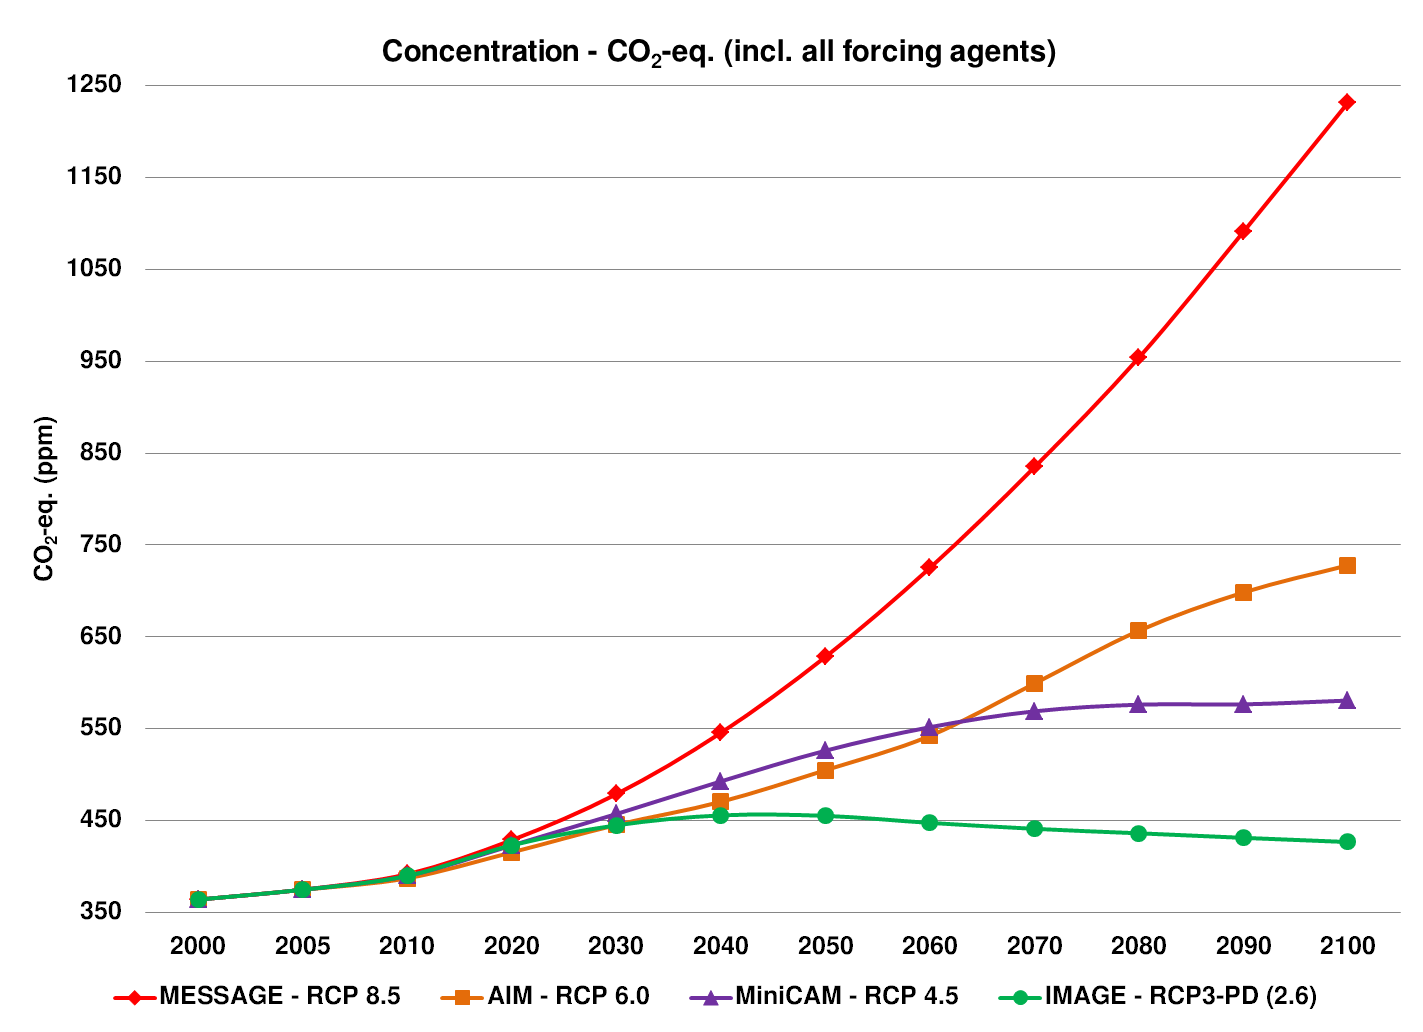
\includegraphics[width=8cm]{CO2-concentration.png}
			\end{figure}
		\end{frame}

	% Slide 4
	\subsection{Climatologías}
	\begin{frame}
		\frametitle{Climatologías}
		\setbeamercovered{transparent}
		\begin{enumerate}[<+(1) | invisible@-+>]
			\item Anuales
			\item Estacionales
			\item Mensuales
		\end{enumerate}
		%\begin{Th2}
%		\begin{figure}[!hbt]
%		   \centering
%		   %\includegraphics[width=3.2 in]{figuras/celdas2.pdf}
%		\end{figure}
		%\end{Th2}
	\end{frame} 

	% Slide 5
%	\subsection{Sistemas de Presión Atmosférica}
%	\begin{frame}
%		\frametitle{Sistemas de Presión Atmosférica [Verano Boreal]}
%		%\begin{Th3}
%		\begin{figure}[!hbt]
%		   \centering
%		   %\includegraphics[width=3.3 in]{figuras/presion1.pdf}
%		\end{figure}
%		%\end{Th3}
%	\end{frame} 

%	% Slide 6
%	\begin{frame}
%		\frametitle{Sistemas de Presión Atmosférica [Verano Austral]}
%		%\begin{Th4}
%		\begin{figure}[!hbt]
%		   \centering
%		   %\includegraphics[width=3.3 in]{figuras/presion.pdf}
%		\end{figure}
%		%\end{Th4}
%	\end{frame} 

	% Slide 7
	\section{Análisis técnico}
	\subsection{Lenguajes/Entornos de programación}
	\begin{frame}
		\frametitle{Lenguajes/Entornos de programación}
		%\begin{Th1}
		\begin{figure}[!hbt]
		   \centering
		   
\includegraphics[width=3.65 in]{mathworks.png}\\
		   
\includegraphics[scale=0.4]{anaconda-python.png}
		\end{figure}
		%\end{Th1}
	\end{frame} 

	% Slide 7
	\subsection{Repositorio de scripts}
	\begin{frame}
		\frametitle{Repositorio de scripts}
		%\begin{Th1}
		\begin{figure}[!hbt]
		   \centering
		   
\includegraphics[width=4 in]{github.png}
		\end{figure}
		\textbf{Link: }\href{https://github.com/cigefi}{https://github.com/cigefi}
		%\end{Th1}
	\end{frame}

	% Slide 8
	\subsubsection{Evolución}
	\begin{frame}
		\frametitle{Evolución}
		\begin{table}
			\captionsetup{labelformat=empty}
			\renewcommand*{\arraystretch}{1.4}
			\renewcommand{\arrayrulecolor}{celeste_ucr}
			\captionsetup{singlelinecheck=false, font=blue, labelfont=sc, labelsep=quad}
			\caption{Línea de tiempo}\vskip -1.5ex
			\begin{tabular}{@{\,}r <{\hskip 2pt} !{\foo} >{\raggedright\arraybackslash}p{8cm}}
				\toprule
				\addlinespace[1.5ex]
				Oct 15 & \textbf{fileOrganize:} re-ordenamiento de la base de datos.\\
				Nov 15 & \textbf{dataProcessing:} descomposición de los datos (mensuales)\\
				Dec 15 & \textbf{dataProcessingERSST:} compactación de datos\\
				Jan 16 & \textbf{climatologies:} climatologías mensuales y estacionales\\
				Feb 16 & \textbf{filesCheck:} revisión de la integridad de los datos\\
				Mar 16 & [...]\\
			\end{tabular}
		\end{table}
	\end{frame}

	% Slide 9
	\section{Resultados}
		\begin{frame}
			\frametitle{Climatologías anuales}
			\begin{figure}[!hbt]
		   		\centering
		   		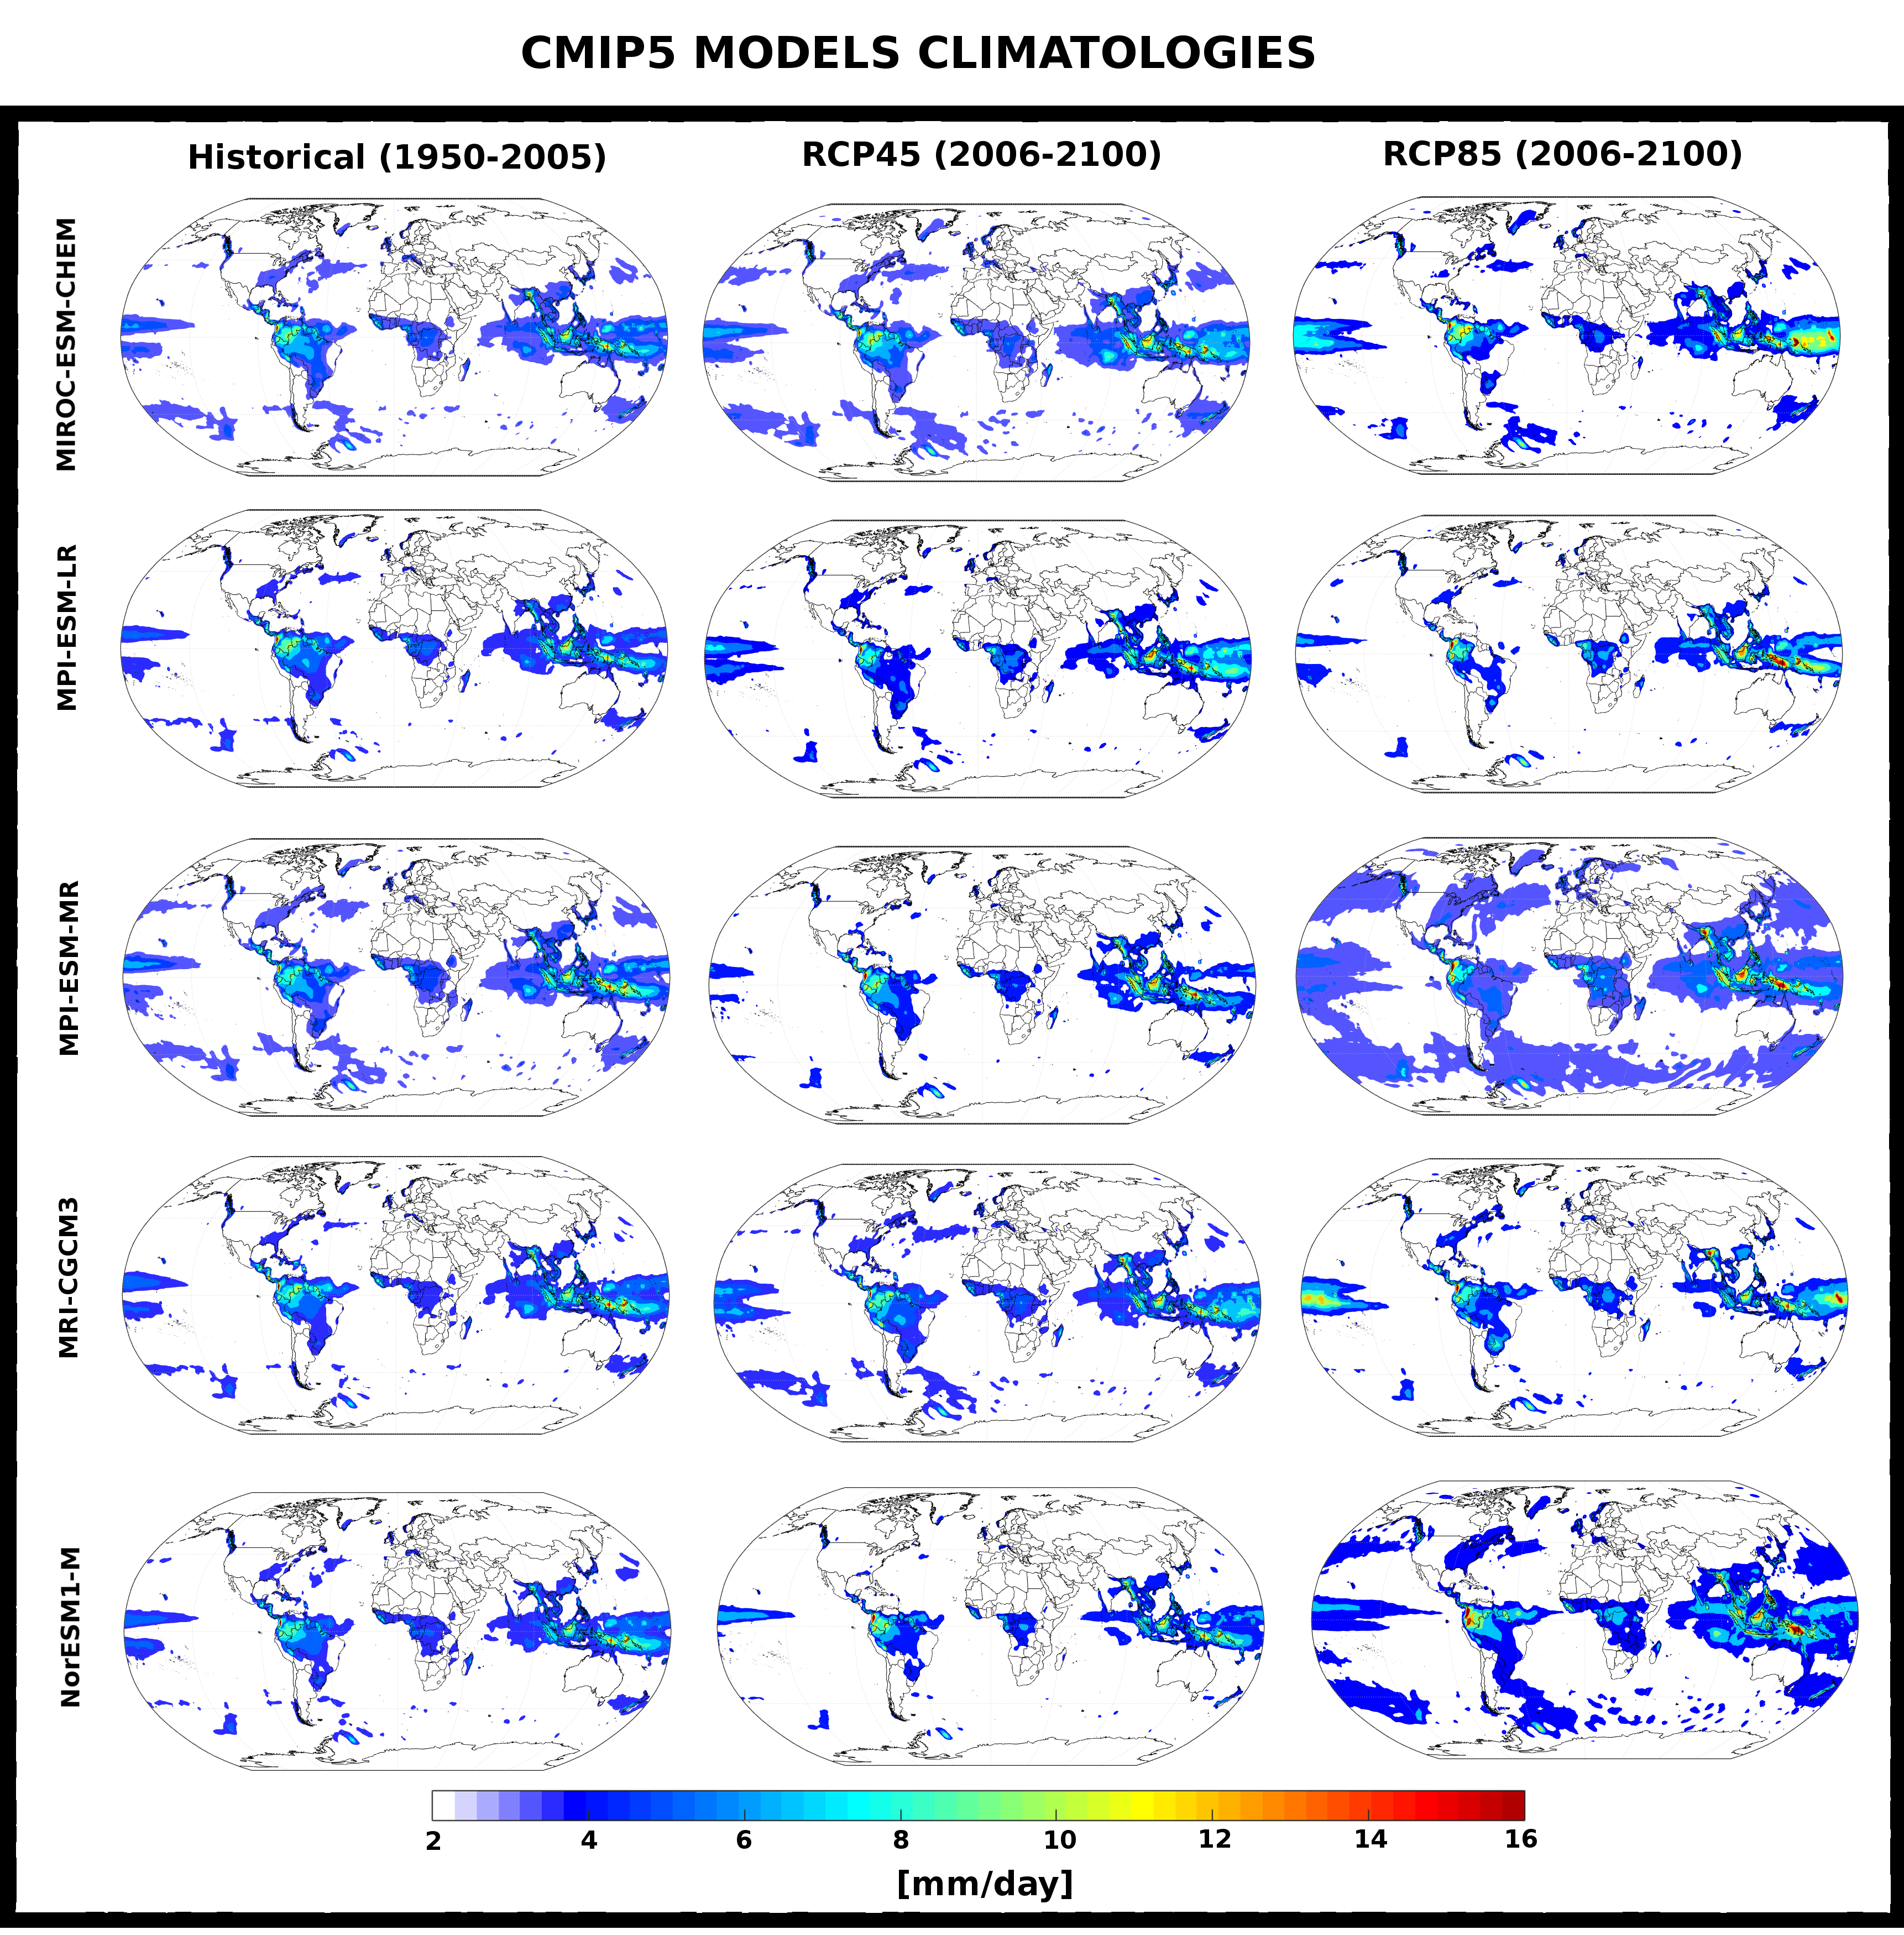
\includegraphics[height=7cm]{graficas.png}
			\end{figure}
		\end{frame}
		
		\begin{frame}
			\frametitle{Climatologías anuales: detalle}
			\begin{figure}[!hbt]
		   		\centering
		   		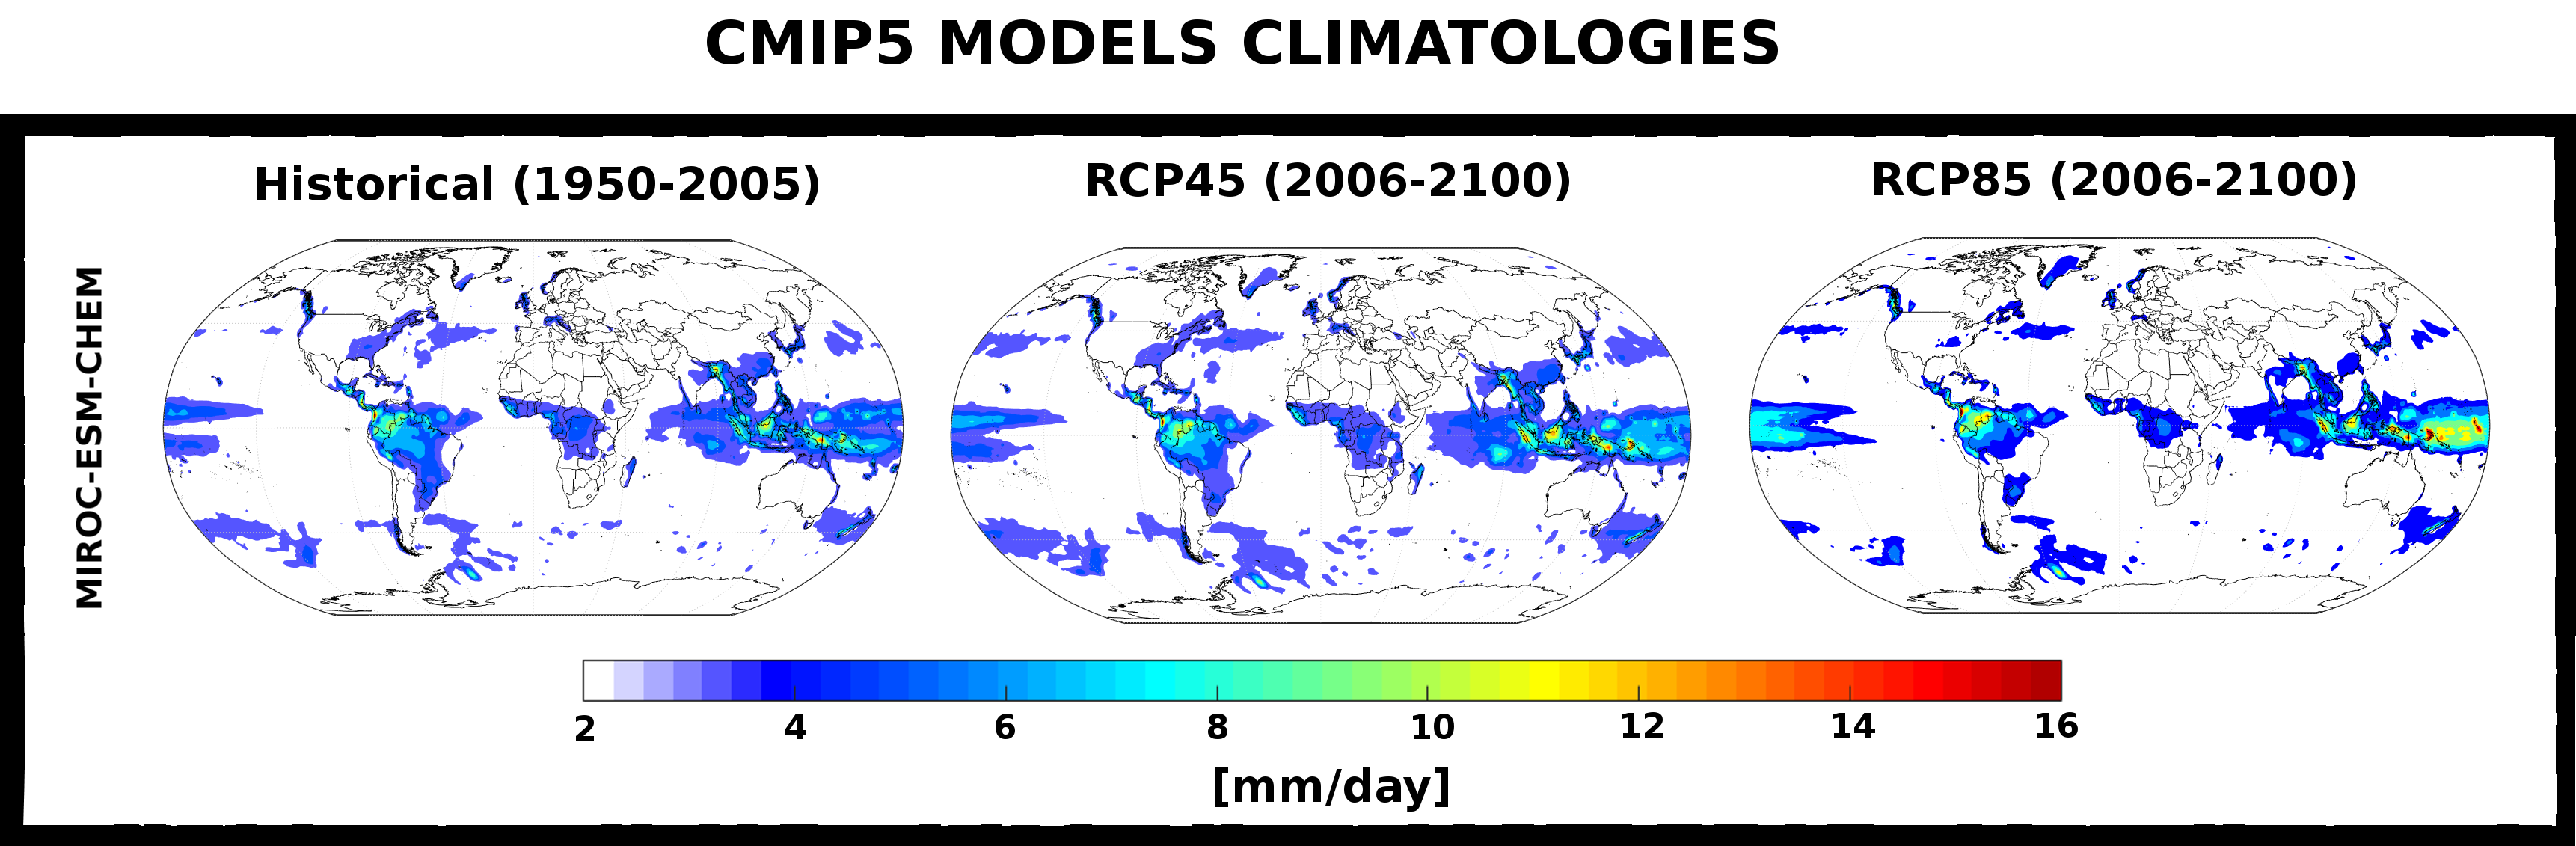
\includegraphics[width=11cm]{detalle-graficas.png}
			\end{figure}
		\end{frame}

	% Slide 13
	\section{Futuros trabajos}
	\subsection{Análisis multivariado (EOF)}
	\begin{frame}
		\frametitle{Análisis multivariado (EOF)}
		\begin{enumerate}
			\item ENSO: El Niño-Southern Oscillation 
			\item NAM: Northern Annular Mode
			\item SAM: Southern Annular Mode
		\end{enumerate}

	\end{frame} 

	% Slide 14
	\begin{frame}
		\begin{center}
			\Huge ¡Muchas gracias!
		\end{center}
	\end{frame}
\end{document} 